\documentclass[12pt]{article}
 
\usepackage[catalan]{babel}
\usepackage[utf8]{inputenc}
\usepackage{float}
\usepackage{hyperref}
\usepackage{listings}

\setlength {\marginparwidth }{2cm}
\usepackage[colorinlistoftodos]{todonotes}

\title{%
Pràctica 1: Inventari d'ens dependents de les Comunitats Autònomes d'Espanya (2017 fins actualitat)\\
\large Tipología i cicle de vida de les dades}
\author{Roger Bosch Mateo}
\date{Octubre de 2019}


\begin{document}

\maketitle

\begin{figure}[H]
    \centering
    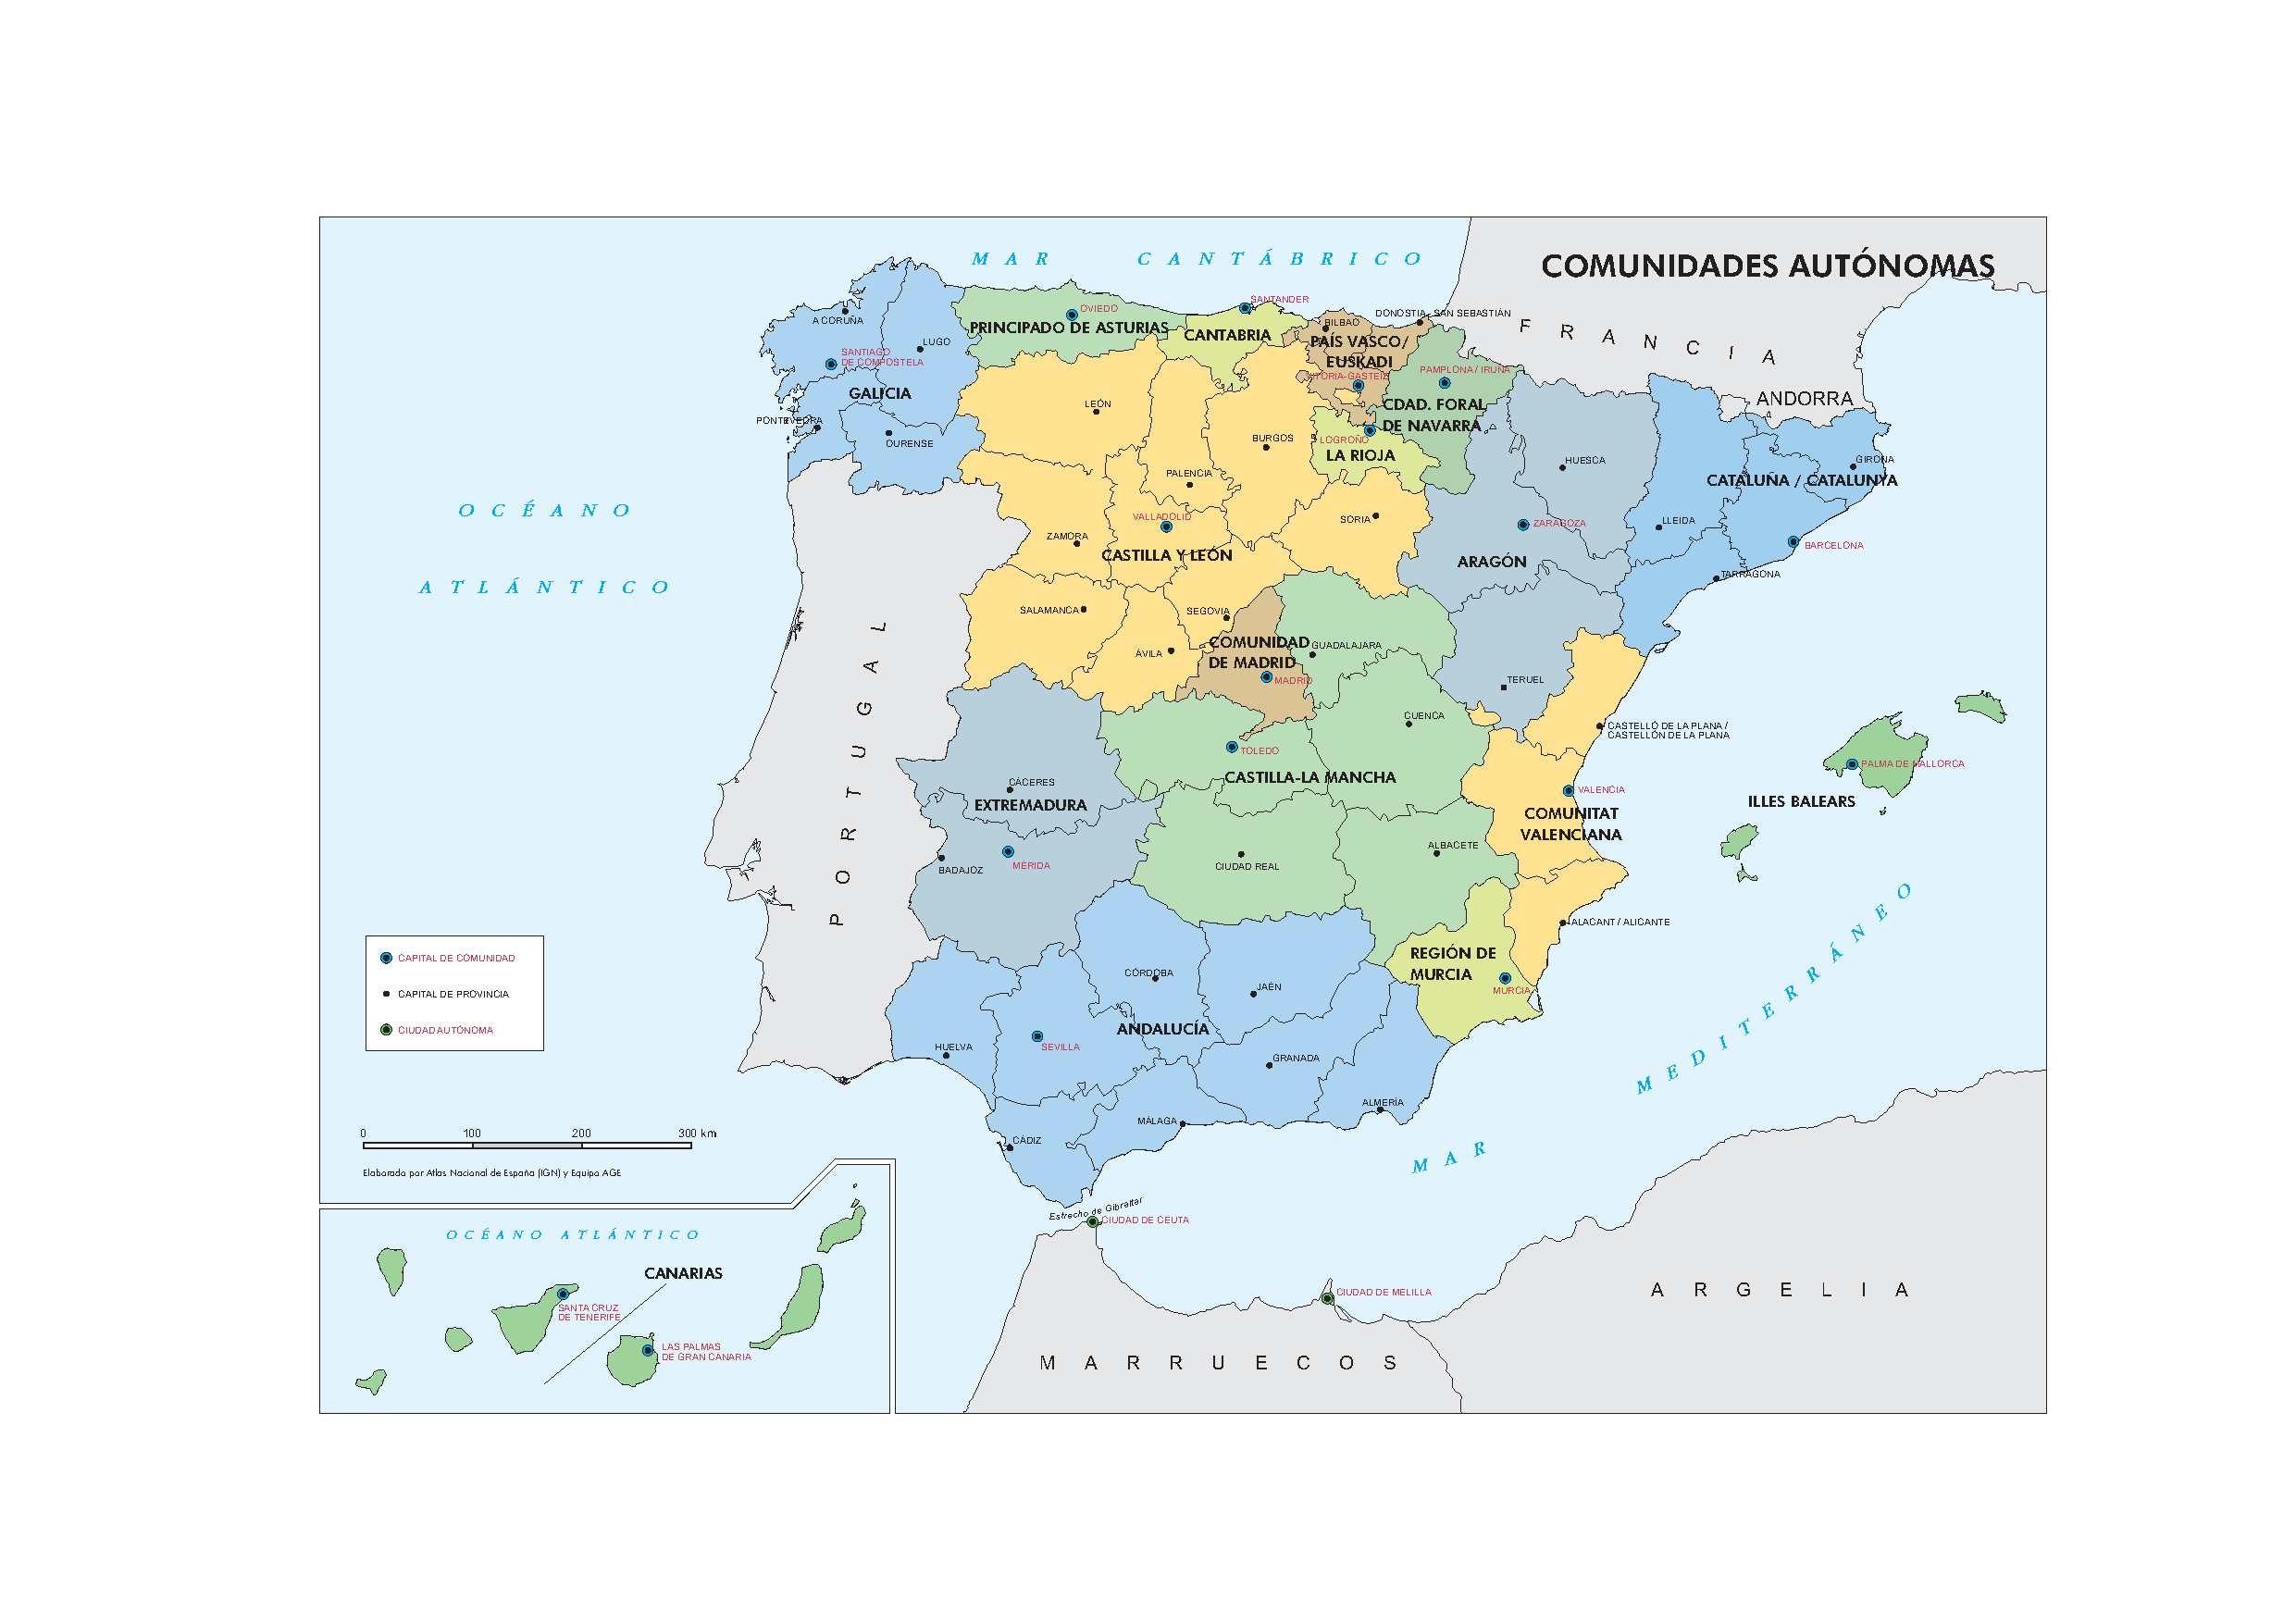
\includegraphics[width=1\columnwidth]{img/mapa.pdf}
    \caption{Comunitats autònomes i províncies d'Espanya} 
    \label{flowchart}
\end{figure}

\section*{Context}
Qualsevol ciutadà té dret a accedir a la informació sobre les diverses activitats públiques del país. La llei 19/2013 de transparència va aconseguir donar un gran pas cap a aquesta fita obligant a les administracions públiques a concedir aquesta informació de manera periòdica, gratuïta, estructurada i reutilitzable entre d'altres. A partir d'aquesta llei són molts els portals oferts per les entitats públiques que faciliten l'accés a tal informació: el portal del Gobern d'Espanya, de Catalunya o de la diputació de Barcelona per posar uns quants exemples.\par
Són tantes les fonts de dades que no totes estan sempre accessibles de la millor manera per l'usuari. 
Un clar exemple és el portal d'\href{https://serviciostelematicosext.hacienda.gob.es/SGCIEF/PubInvCCAA/secciones/FrmSelComunidad.aspx}{inventaris d'ens dependents de les comunitats autònomes} que permet únicament la visualització de l'informació de manera individual i en cap moment es pot descarregar, dificultant així l'accés a dita informació.
Aquest \textit{dataset} preten posar un petit gra de sorra per facilitar al ciutadà un accés de qualitat a la informació del portal.

\section*{Descripció del \textit{dataset}}
El portal d'\href{https://serviciostelematicosext.hacienda.gob.es/SGCIEF/PubInvCCAA/secciones/FrmSelComunidad.aspx}{inventaris d'ens dependents de les comunitats autònomes} mostra informació de les 16 comunitats autònomes (Andalusia, Aragó, Principat d'Astúries, Illes Balears, País Basc, Canàries, Cantabria, Castella la Manxa, Castella i Lleó, Catalunya, Extremadura, Galícia, Comunitat de Madrid, Regió de Múrcia, Navarra, La Rioja i País Valencià) i les dues ciutats autònomes (Ceuta i Melilla) d'Espanya. Per a cada comunitat autònoma, es mostren totes aquelles entitats que es consideren integrants de l'inventari d'ens de cada comunitat autònoma (Autogobern de la comunitat autònoma, organismes autònoms administratius, organismes autònoms comercials, organismes autònoms, entitats públiques empresarials, ens públics, consorcis, fundacions, altres institucions sense ànim de lucre, societats mercantils i universitats). Per a cada entitat es mostra informació, si existeix: de caràcter general, de les activitats que realitza, dels components que la formen, l'històric de noms oficials i de capital social.\par

\section*{Contingut}

El dataset inclou cinc taules diferents: dades generals, activitats, components (i components alternatiu), històric de noms i històric de capital social. És a dir, no estem parlant d'un dataset amb un únic fitxer CSV que el pot representar ja que hi ha diverses relacions entre aquestes taules. En la Figura \ref{UML} es poden veure les associacions entre cadascuna d'aquestes taules.


\begin{figure}[H]
    \centering
    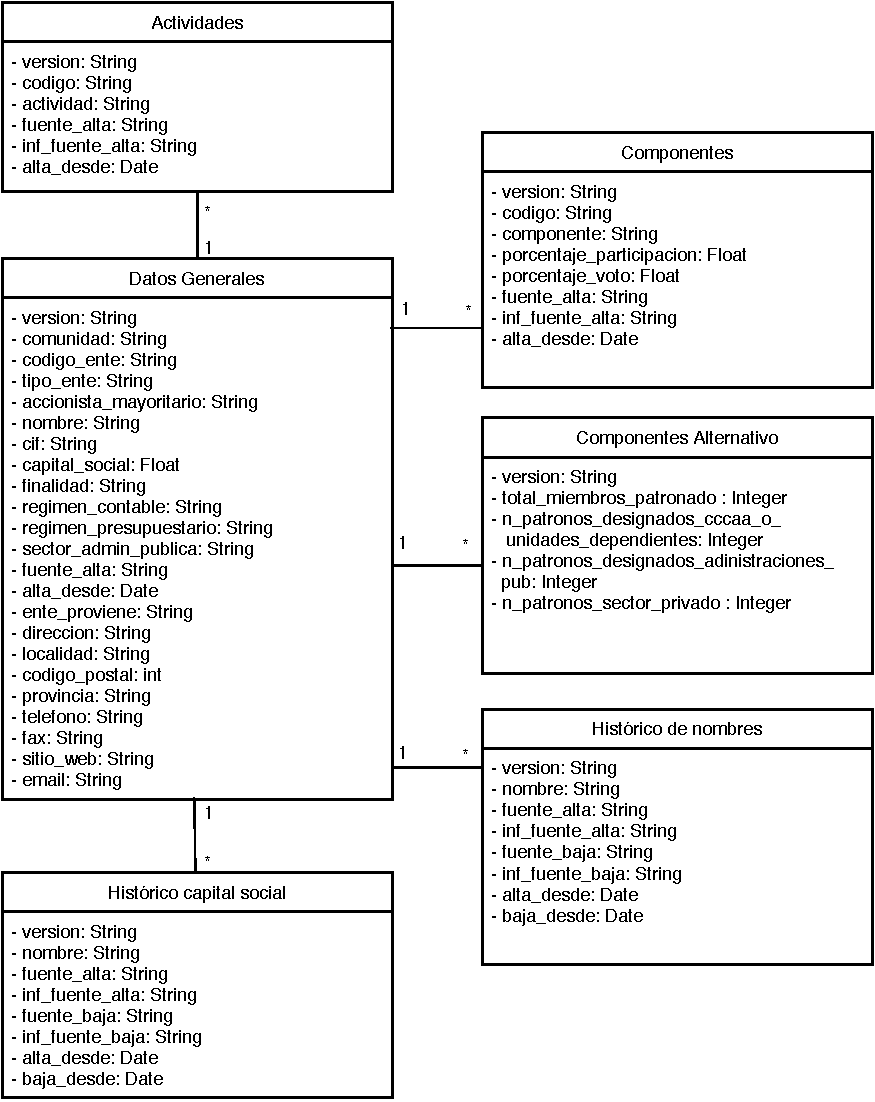
\includegraphics[width=0.7\columnwidth]{img/UML.pdf}
    \caption{Esquema UML} 
    \label{UML}
\end{figure}


Cal mencionar que per a cadascun dels ens hi ha la possibilitat de visualitzar la informació històrica, és a dir, veure la informació que hi havia sobre un ens en una data concreta. És per aixó que cadascuna de les taules presenta l'atribut \textit{version} que donta quina versió de les dades s'està utilitzan segons la pàgina web.
Seguidament per a cadascuna de les taules es descriuen els seus atributs:
\paragraph{Datos generales\\}
\begin{itemize}
    \item \textbf{version}: Indica la versió que representa la informació. Usualment cada any presenta dues versions diferents la 01 i la 02. És per aixó que sol tenir els valors 200XX/0X.
    \item \textbf{comunidad}: Nom de la comunitat autònoma a la que pertany l'entitat.
    \item \textbf{codigo\_ente}: Codi identificador de l'entitat.
    \item \textbf{tipo\_ente}: Indica la tipología de l'entitat segons la classificació esmentada en el README.md.
    \item \textbf{accionista\_mayoritario}: Nom de l'entitat accionista majoritària si n'hi ha.
    \item \textbf{nombre}: Nom de l'entitat.
    \item \textbf{cif}: Identificador CIF de l'entitat.
    \item \textbf{capital\_social}: Capital social de l'entitat. Pot ser nul.
    \item \textbf{finalidad}: Correspon a la finalitat insitucional, estatutària o societària atribuida a cada entitat.
    \item \textbf{regimen\_contable}: Indica el règim contable al que queda subjecte l'entiat.
    \item \textbf{regimen\_presupuestario}: Fa referència al règim pressupostari aplicable a la entitat conforme a les normes aplicades.
    \item \textbf{sector\_admin\_publica}: Ofereix informació sobre la sectorització que, en el moment de la publicació, tenen vigents les entitats.
    \item \textbf{fuente\_alta}: Informació d'alta de l'entitat a l'inventari.
    \item \textbf{alta\_desde}: Data d'alta de l'entitat.
    \item \textbf{ente\_proviene}: Per aquelles entitats que tenen l'origen en una altre entitat, n'indica el nom d'aquesta.
    \item \textbf{direccion}: Indica la direcció de l'entitat.
    \item \textbf{localidad}: Indica la localitat on està situada l'entitat.
    \item \textbf{codigo\_postal}: Indica el codi postal de la localitat de l'entitat.
    \item \textbf{provincia}: Indica la província on està situada l'entitat.
    \item \textbf{telefono}: Indica el telèfon de l'entitat.
    \item \textbf{fax}: Indica el fax de l'entitat.
    \item \textbf{sitio\_web}: Indica la pàgina web de l'entitat.
    \item \textbf{email}:  Indica el correu electrònic de l'entitat.
\end{itemize}

\paragraph{Actividades\\}
\begin{itemize}
    \item \textbf{version}: Indica la versió que representa la informació. Usualment cada any presenta dues versions diferents la 01 i la 02. És per aixó que sol tenir els valors 200XX/0X.
    \item \textbf{codigo\_ente}: Codi identificador de l'entitat.
    \item \textbf{codigo}: Codi CNAE corresponent a l'activitat.
    \item \textbf{actividad}: Nom de l'activitat.
    \item \textbf{fuente\_alta}: Data d'alta d'aquesta activitat de l'entitat a l'inventari.
    \item \textbf{inf\_fuente\_alta}: Informació sobre l'alta de l'activitat.
    \item \textbf{alta\_desde}: Data d'alta oficial d'aquesta activitat a l'entitat.
\end{itemize}

\paragraph{Componentes\\}
\begin{itemize}
    \item \textbf{version}: Indica la versió que representa la informació. Usualment cada any presenta dues versions diferents la 01 i la 02. És per aixó que sol tenir els valors 200XX/0X.
    \item \textbf{codigo\_ente}: Codi identificador de l'entitat.
    \item \textbf{codigo}: Codi del component (entitat) que forma part d'aquesta entitat.
    \item \textbf{componente}: Nom del component.
    \item \textbf{porcentaje\_participacion}: Percentatge de participació que ostenta cada component sobre aquesta entitat.
    \item \textbf{porcentaje\_voto}: Percentatge de vot directe que ostenta cada component sobre aquesta entitat.
    \item \textbf{fuente\_alta}: Data d'alta d'aquest component de l'entitat a l'inventari.
    \item \textbf{inf\_fuente\_alta}: Informació sobre l'alta del component.
    \item \textbf{alta\_desde}: Data d'alta oficial d'aquest component a l'entitat.
\end{itemize}

\paragraph{Componentes alternativo\\}
\begin{itemize}
    \item \textbf{version}: Indica la versió que representa la informació. Usualment cada any presenta dues versions diferents la 01 i la 02. És per aixó que sol tenir els valors 200XX/0X.
    \item \textbf{codigo\_ente}: Codi identificador de l'entitat.
    \item \textbf{total\_miembros\_patronado}: Nombre total de membres del patronat.
    \item \textbf{n\_patronos\_designados\_cccaa\_o\_unidades\_dependientes}: Nombre de membres del patronat designats per la comunitat autònoma o per alguna de les seves unitats dependents.
    \item \textbf{n\_patronos\_designados\_adinistraciones\_pub}: Nombre de membres del patronat designats per altres administracions públiques.
    \item \textbf{n\_patronos\_sector\_privado}: Número de patrons designats pel sector privat.
\end{itemize}

\paragraph{Histórico de nombres\\}
\begin{itemize}
    \item \textbf{version}: Indica la versió que representa la informació. Usualment cada any presenta dues versions diferents la 01 i la 02. És per aixó que sol tenir els valors 200XX/0X.
    \item \textbf{codigo\_ente}: Codi identificador de l'entitat.
    \item \textbf{nombre}: Nom assignat.
    \item \textbf{fuente\_alta}: Data d'alta d'aquest nom de l'entitat a l'inventari.
    \item \textbf{inf\_fuente\_alta}: Informació sobre l'alta del nom.
    \item \textbf{fuente\_baja}: Data de baixa d'aquest nom de l'entitat a l'inventari.
    \item \textbf{inf\_fuente\_baja}: Informació sobre la baixa del nom.
    \item \textbf{alta\_desde}: Data d'alta oficial d'aquest nom a l'entitat.
    \item \textbf{baja\_desde}: Data de baixa oficial d'aquest nom a l'entitat.
\end{itemize}
\paragraph{Histórico capital social\\}
\begin{itemize}
    \item \textbf{version}: Indica la versió que representa la informació. Usualment cada any presenta dues versions diferents la 01 i la 02. És per aixó que sol tenir els valors 200XX/0X.
    \item \textbf{codigo\_ente}: Codi identificador de l'entitat.
    \item \textbf{capital\_social}: Valor del capital social de l'entitat.
    \item \textbf{fuente\_alta}: Data d'alta d'aquest capital social de l'entitat a l'inventari.
    \item \textbf{inf\_fuente\_alta}: Informació sobre l'alta del capital social.
    \item \textbf{fuente\_baja}: Data de baixa d'aquest capital social de l'entitat a l'inventari.
    \item \textbf{inf\_fuente\_baja}: Informació sobre la baixa del nom.
    \item \textbf{alta\_desde}: Data d'alta oficial d'aquest capital social a l'entitat.
    \item \textbf{baja\_desde}: Data de baixa oficial d'aquest capital social a l'entitat.
\end{itemize}

\begin{figure}[H]
    \centering
    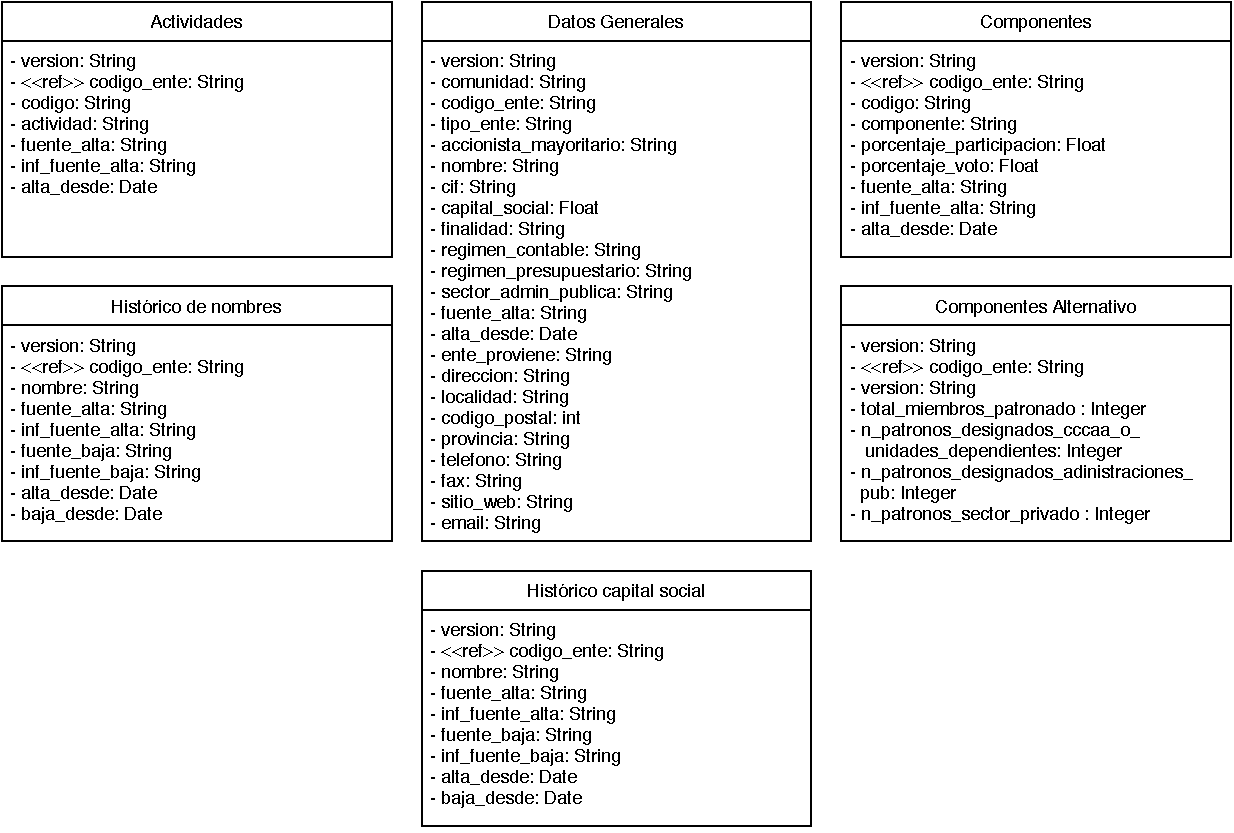
\includegraphics[width=0.7\columnwidth]{img/diagrama_classes_entitat.pdf}
    \caption{Diagrama de classes d'entitat} 
    \label{clasesentitat}
\end{figure}

\section*{Solució tencològica}
El portal web permet a l'usuari veure un per un per cada comunitat autònoma totes les entitats associades. A més d'un llistat genèric el portal proporciona un cercador, però aquest no és gens senzill d'utilitzar. Primer de tot perquè si vols veure els resultats de dues comunitats autònomes no pots: primer has de buscar-ne un i després l'altre. Segon, perquè els camps de cerca no són gens entenedors per un usuari casual fet que dificulta la feina a l'usuari.\par

Aquest \textit{web scraper} creat facilita l'extracció de tota l'informació del portal utilitzant \textbf{Selenium}\footnote{\url{https://selenium-python.readthedocs.io/installation.html}} per a Python. En la Figura \ref{flowchart} es pot veure el fluxe que es segueix per a la realització de l'scraping.

\begin{figure}[H]
    \centering
    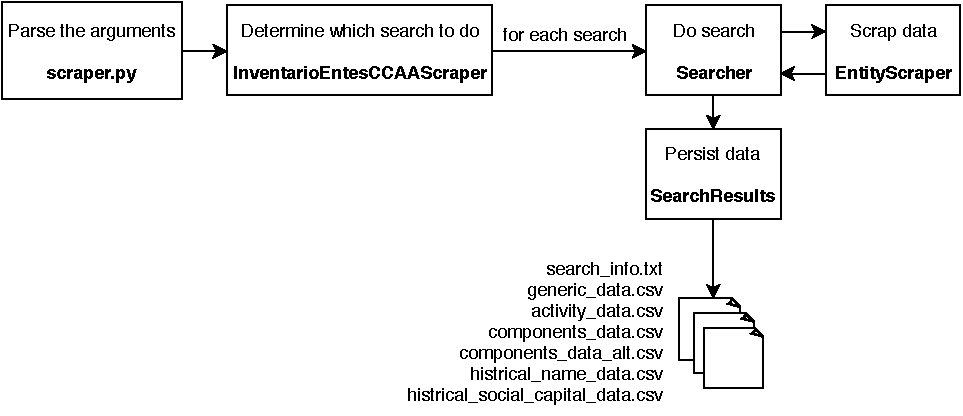
\includegraphics[width=1\columnwidth]{img/flowchart.pdf}
    \caption{Fluxe de l'scraping} 
    \label{flowchart}
\end{figure}

\begin{itemize}
    \item \textbf{scraper.py}: És el fitxer que ha de cridar l'usuari per iniciar l'scraping. Admet una gran varietat de configuracions que permeten a l'usuari realitzar cerques d'una manera molt més senzilla que en el portal sense haver-se de preocupar de res. L'usuari podrà introduir la comunitat autònoma, província o tipus d'entitat entre d'altres i el programa se'n encarregarà de realitzar-lo. Hi ha una certa complexitat en les configuracions, i no ha sigut una tasca senzilla ja que en el portal no es mostra en cap moment informació sobre els camps que en tot moment són numèrics. Una descripció detallada dels arguments suportats amb exemples està disponible en el \textbf{README.md} del \href{https://github.com/boschmateo/InventarioEntesCCAA}{repositori} de Github.
    \item \textbf{InventarioEntesCCAAScraper}: Una vegada tenim tots els arguments que defineixen la cerca que l'usuari desitja, s'han d'interpretar. Aquesta classe prendrà tots els arguments i determinarà quantes cerques s'han de realitzar i amb quins arguments. Per exemple un usuari en una mateixa cerca pot voler buscar informació sobre les societats mercantils i les universitats de la comunitat autònoma de Catalunya i la província de Viscaya. Per obtenir els resultats d'aquesta informació s'han de realitzar un total de 10 cerques degut a les limitacions del cercador:
    \begin{itemize}
        \item Les societats mercantils tenen quatre representacions en codi\footnote{Tots aquests codis no estan especificats en cap lloc del portal i han sigut extrets manualment a base de cerques.} segons les seves característiques "B-P", "X-P", "Z-P" i "F-P". Per cada tipus hem de realitzar una cerca diferents i tenim dues comunitats autònomes a cercar que són Catalunya i el País Vasc (on pertany Viscaya). Per tant amb les societats mercantils s'han de realitzar vuit cerques diferents.
        \item Les universitats estan representades únicament amb el codi "B-W" i com tenim Catalunya i Viscaya hem de fer dues cerques més, fent un total de deu cerques.
    \end{itemize}
    En aquest punt cal considerar que l'\textit{input} rebut per part de l'usuari és textual, mentre que el portal únicament accepta un codi preestablert. És per això que en aquest punt també es transformen els valors textuals als codis numèrics corresponents gràcies a l'investigació del significats d'aquests, com per exemple amb la traducció del nom de les províncies al seu codi \cite{INE}.
    \item \textbf{Searcher}: Aquest clase prendrà els arguments definitius d'una de les cerques a realitzar: quina comunitat autònoma ha de seleccionar, quina versió o quin tipus d'entitat entre d'altres. Quan hagi introduit tots els valors realitzarà la cerca, n'extreurà tots els links a les entitats a obtenir informació i per cadascun dels enllaços invocarà a \textit{EntityScraper} perquè n'extregui la informació.
    \item \textbf{EntityScraper}: A partir del link realitzarà un \textit{request} i n'extraurà la informació disponible per aquesta entitat. En aquest punt cal esmentar que tot i que en la majoria dels casos l'estructura és la mateixa, en algunes entitats aquesta canvia. És el cas de l'informació genèrica que en alguns casos és mostra desordenada i per tant el \textit{path} al valors dels atributs és diferent i el cas de la taula "\textit{Components}" que a vegades mostra informació completament diferent (és per això que s'ha creat la taula \textit{components\_alt\_data}).
    \item \textbf{SearchResults}: Finalment s'exporten totes les dades en un total de sis fitxers diferents seguint l'estructura presentada en la Figura \ref{clasesentitat}. També crea el fitxer \textit{search\_info.txt} que conté informació de cadascuna de les cerques realitzades per obtenir l'informació final. Aquest fitxer és molt útil a mode de traçabilitat dels resultats.
\end{itemize}


\section*{Tècniques per evitar el bloqueig}
Tot i que no es va trobar cap problema de bloqueig durant el web scraping inicial, s'han decidit aplicar algunes tècniques per evitar ser bloquejats durant l'utilització del scraper.
\begin{itemize}
    \item Amb l'ús de \textit{User-Agent Spoofing} cada vegada que es realitza un \textit{request} el \textit{header} és cambiat per un altre totalment diferent, gràcies a la llibreria de Python \texttt{fake-useragent}\footnote{\url{https://pypi.org/project/fake-useragent/}} que proporciona una base de dades amb dades reals. 
    \item Per evitar saturar el servidor es calcula el temps que s'ha tardat en rebre l'últim \textit{request} realitzat i no es realitza el següent fins que hagin passat deu vegades aquest temps.
    \item El comportament de l'scraping varia en certs punts:
    \begin{itemize}
        \item Quan la classe \textit{InventarioEntesCCAAScraper} determina quines cerques s'han de realitzar, aquestes no es realitzen seqüencialment sinó de manera aleatòria. Seguint l'exemple donat si no es realitzes aleatoriament primer es realitzarien totes les cerques de Catalunya i després les del País Vasc. Al aleatoritzar-ho fem que aquestes s'intercalin evitant així realitzar sempre el mateix ordre.
        \item La mateixa acció realitza la clase \textit{Searcher} al cridar \textit{EntityScraper}. Els links no es seguixen seqüencialment.
    \end{itemize}
\end{itemize}

Per a fer-ho possible s'ha creat un \textit{wrapper} cada vegada que es fa una crida al driver de selenium que obliga a realitzar l'espera tal i com es mostra en el següent codi. L'únic que s'ha de fer des de l'scraper és cridar al mètode \texttt{get()} amb la \texttt{url} desitjada.




\noindent\begin{lstlisting}[language=Python]
    def get(self, url):
      # If it's the first request no restrictions 
      # are set
      if self.latest_response_delay is None:
        self._get(url)
      # Otherwise
      else:
        # Wait 10 times the time it took to do 
        # the latest request
        while time.time() - self.latest_request_time
        < 10*self.latest_response_delay:
          time.sleep(0.1)
        # Call function to do the request
        self._get(url)

    def _get(self, url):
      # Randomize the user-agent header
      self.driver.execute_cdp_cmd(
        'Network.setUserAgentOverride', 
        {"userAgent": self.ua.random}
        )

      # Calculate the time it elapses between the 
      # start of the request and the end
      start = time.time()
      self.driver.get(url)
      self.latest_response_delay = time.time() - start
      self.latest_request_time = time.time()
\end{lstlisting}




\section*{Agraïments}
Els propietaris d'aquestes dades són les comunitats i ciutats autònomes i l'Administració General de l'Estat. Les dades recollides en l'inventari són subministrades per totes les comunitats i ciutats autònomes a la "Direcció General de Coordinació Finançera amb les Comunitats Autònomes" els quals mantenen aquestes dades actualitzades permanentment en el portal \cite{PDFAjuda}.

\section*{Inspiració}
Aquest \textit{dataset} és de gran interés per entendre millor les comunitats autònomes. De manera global a tota Espanya i per cada comunitat autònoma podem estudiar tots els ens dels que disposa i obtenir informació interessant sobre aquesta:
\begin{itemize}
    \item Quantes entitats dependents de les comunitats autònomes hi ha? Quin tipus d'entitats predominen globalment, en cada comunitat, en cada província o fins i tot en cada ciutat?
    \item Quina comunitat autònoma presenta a dia d'avuí més capital social segons totes les seves entitats i com ha anat evolucionant des de 2007 fins a l'actualitat?
    \item Quin tipus d'entitat sol presentar més canvis de nom al llarg de la història? Són canvis de nom significatius o petites variacions?
    \item Hi ha algú que tingui participació en diverses entitats? Té el control sobre aquestes (més 50\%) o no?
    \item A més, permet obtenir informació de contacte de cada entitat (telèfon, pàgina web, correu electònic...) i el seu identificador (cif), que pot ser utilitzat per agregar dades d'altres fonts d'informació.
\end{itemize}

Cal dir que aquests són només uns quants exemples de preguntes que podrien ser respostes amb el dataset, però de ben segur que a mesura que aquestes es responen moltes altres preguntes de gran interès sorgeixen.


\section*{Llicència}
La llicència resultant sobre la que es llibera el \textit{dataset} és \textit{\textbf{Public Domain License (CC0)}}, perquè qualsevol individu pugui copiar, modificar, distribuit i fer comunicació pública d'aquesta fins i tot per fins comercials.
Aquesta el·lecció es basa en la naturalesa de les dades i l'\textit{Open Data}. Com ja s'ha comentat qualsevol individu ha de tenir accés a aquesta informació de caràcter públic i aquest \textit{dataset} és un pas cap a aquest objectiu permetent de manera senzilla la reutilització d'aquestes dades, cosa que el portal no permet.

\newpage
\section*{Contribucions}
Les contribucions en aquest projecte són les següents:
\begin{table}[h!]
    \centering
     \begin{tabular}{p{5cm}p{5cm}} 
     \hline
     \textbf{Contribucions} & \textbf{Signa} \\
     \hline
     Recerca prèvia & Roger Bosch Mateo \\
     Redacció de respostes & Roger Bosch Mateo \\
     Desenvolupament codi & Roger Bosch Mateo \\
     \hline
    \end{tabular}
    \caption{Taula de contribucions al projecte}
    \label{ComparativaAPITwitter}
\end{table}

\newpage
\begin{thebibliography}{9}
    \bibitem{INE} 
    "Relación de provincias con sus códigos", Instituto Nacional de Estadística (INE). Obtingut de \url{https://www.ine.es/daco/daco42/codmun/cod_provincia.htm}
    \bibitem{PDFAjuda} 
    "Notas relativas a la información contenida en el inventario de entes integrantes de las comunidades autónomas". Obtingut de \url{https://serviciostelematicosext.hacienda.gob.es/SGCIEF/PubInvCCAA/Ayuda/NOTAS\%20INFORMATIVAS.pdf}
\end{thebibliography}

\end{document}
